\documentclass[12pt]{exam}
\usepackage[phy]{template-for-exam}
\usepackage{tikz,ifthen,multicol,siunitx}
\footer{}{}{}
\header{}{}{}
\shadedsolutions
\printanswers
\usetikzlibrary{shadings,decorations.pathmorphing,arrows.meta,patterns}



\begin{document}

\Large

\def\mystrut{\protect\rule[-2.2ex]{0ex}{2.2ex}} 
\qformat{ \textbf{Task \#\thequestion}
  \mystrut  \hfill}


\begin{questions}

  \vspace*{\stretch{1}}


\question
  Consider the folowing objects that collide on a frictionless surface.  If $m_A=4$ kg and $m_B=1$ kg, what is the final velocity of object A?

  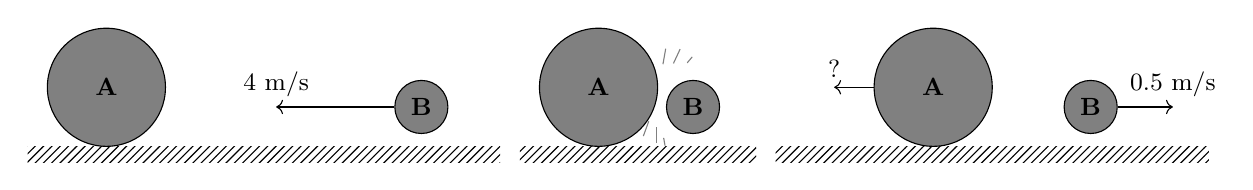
\begin{tikzpicture}
    \begin{scope}
      \node
        [circle, minimum size=1.5cm, fill=gray, draw=black] 
        at (0,.25) (A) {\small \bf A};
      \node[circle, fill=gray, draw=black] 
        at (4,0) (B) {\small \bf B};
      \draw[->] (B.west) -- ++(-1.5,0) 
        node[above] {\small 4 m/s};
      \fill[pattern=north east lines]
        (-1,-0.5) rectangle ++(6,-0.2);
    \end{scope}

    \begin{scope}[shift={(6.25,0)}]
      \node
        [circle, minimum size=1.5cm, fill=gray, draw=black] 
        at (0,.25) (A) {\small \bf A};
      \node[circle, fill=gray, draw=black] 
        at (1.2,0) (B) {\small \bf B};
      \fill[pattern=north east lines]
        (-1,-0.5) rectangle ++(3,-0.2);

        \begin{scope}[shift={(.74,0.1)},gray]
          \draw[] (50:.6) -- ++(50:.1);
          \draw[] (65:.5) -- ++(65:.2);
          \draw[] (80:.45) -- ++(80:.2);
          \draw[] (-80:.5) -- ++(-80:.1);
          \draw[] (-90:.36) -- ++(-90:.2);
          \draw[] (-110:.3) -- ++(-110:.2);
        \end{scope}
    \end{scope}

    \begin{scope}[shift={(9.5,0)}]
      \node
        [circle, minimum size=1.5cm, fill=gray, draw=black] 
        at (1,.25) (A) {\small \bf A};
      \node[circle, fill=gray, draw=black] 
        at (3,0) (B) {\small \bf B};
      \draw[->] (B.east) -- ++(.7,0) 
        node[above] {\small 0.5 m/s};
      \draw[->] (A.west) -- ++(-.5,0) 
        node[above] {\small ?};
      \fill[pattern=north east lines]
        (-1,-0.5) rectangle ++(5.5,-0.2);
    \end{scope}
  \end{tikzpicture}

\vs \hrule \vs

\question
  A 1500-kg truck traveling at 15~m/s rear-ends a stationary 900-kg car.  After the collision, the two vehicles stick together.  Before friction has a chance to take effect, what is the speed of the cars?


\vs \hrule \vs

\question
  A 900-kg cannon fires a 5-kg cannonball at a speed of 30~m/s.  What is the speed of the cannon's recoil?

  \vs 




\end{questions}




\end{document}